\documentclass[pdf]{beamer}
%\documentclass[notes]{beamer}
%\documentclass{beamer}
\usepackage[utf8]{inputenc}
\usepackage{lmodern}
\usepackage{colortbl}
\usepackage{adjustbox}
%\usepackage{scrextend}
%\changefontsizes{7.5pt}


\makeatletter
\makeatother
\usepackage{graphicx}

\mode<presentation>{\usetheme{Warsaw}}
%\mode<presentation>{\usetheme{Madrid}}
%% preamble
\title{Métodos multivariados de Análisis de Datos}
\subtitle{Análisis de nutrientes en pizzas}

\author{
Ricardo Cruz Sánchez \\
  \and
Rolando Corona Jiménez
}

\institute[CIMAT]{CIMAT}


\begin{document}

\begin{frame}
\titlepage
\end{frame}

%\AtBeginSubsection[]
%{
%  \begin{frame}<beamer>
%    \frametitle{Contenido}
%    \tableofcontents[currentsection,currentsubsection]
%  \end{frame}
%}

\section{Resumen}

\begin{frame}{Resumen}
\begin{enumerate}
\item primeros lugares en morbilidad y mortalidad a nivel mundial.
\item la hiperglucemia causa alteraciones en el metabolismo de la glucosa y l\'ipidos.
\item El padecimiento es cr\'onico-degenerativo
\item Desde el a\~no 2000, la diabetes mellitus en M\'exico es la primera causa de muerte entre las mujeres y la segunda entre los hombres
\item la edad, la obesidad, el sedentarismo, la alimentación inadecuada, los antecedentes familiares y algunos factores gen\'eticos
\item detección temprana
\item Incorporación de base de conocimiento en RB.
\end{enumerate}
\end{frame}


\section{Proposito y objetivos}
\begin{frame}{Proposito y objetivos}
\begin{block}{Objetivo general}
Generar un modelo confiable con el cual se pueda detectar de manera eficiente, econ\'omica y sencilla la presencia de DM2 en la población mexicana femenina.
\end{block}

\begin{block}{objetivo secundario}
\begin{enumerate}
	\item Incorporar a la poblaci\'on masculina en el estudio.
	\item Crear política públicas encaminadas a erradicar el padecimiento con base en los resultados generados por el modelo.
	\item Disminuir los costos que se generan en los centros de salud causados por la detecci\'on tard\'ia de DM2
\end{enumerate}
\end{block}
\end{frame}

\section{Modelos de reducción de dimensiones.}

\subsection{Análisis de componentes principales (PCA)}

\begin{frame}{Cargas de componentes principales}
\begin{table}[ht]
\centering
\begin{tabular}{rrr}
  \hline
 & PC1 & PC2 \\ 
  \hline
Humedad & 0.21 & 0.58 \\ 
  Proteina & -0.47 & -0.03 \\ 
  Grasa & -0.19 & 0.41 \\ 
  Ceniza & -0.51 & 0.15 \\ 
  Sodio & -0.47 & -0.02 \\ 
  Carbohidratos & 0.32 & -0.49 \\ 
  Calorias & -0.34 & -0.48 \\ 
  Varianza acumulada & 48.64 \% &  83.59 \% \\ 
\end{tabular}
	\label{tabla:pesos_PCA}
	\caption{Pesos asociados a las primeras dos componentes principales.}
\end{table}
\end{frame}


\begin{frame}
\begin{figure}[h]
\centering
	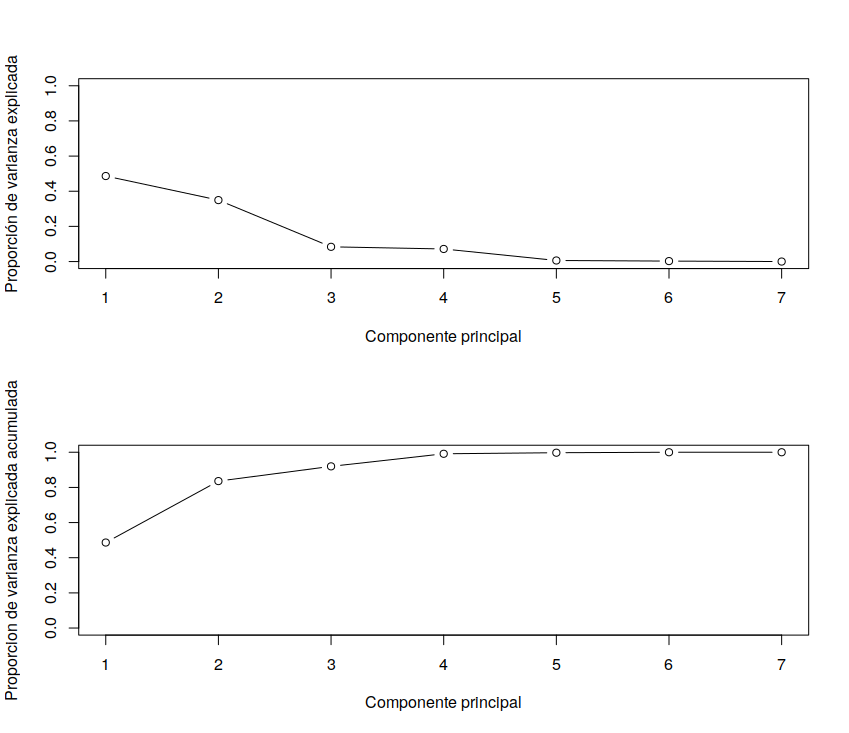
\includegraphics[scale=.35]{images/varPCA.png} 
	\label{i_var_PCA}
	\caption{Varianza explicada por las componentes principales}
\end{figure}
\end{frame}


\begin{frame}
\begin{figure}[h]
\centering
	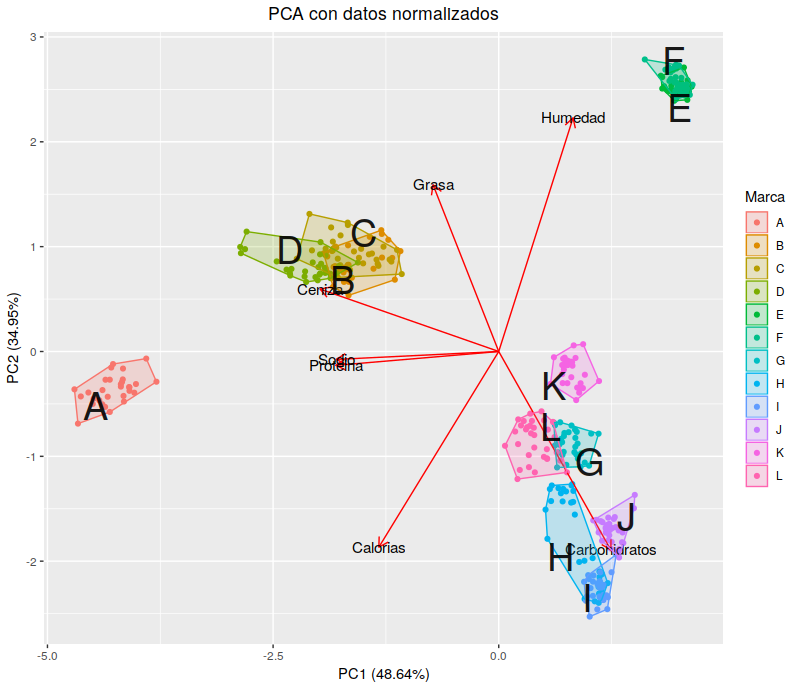
\includegraphics[scale=.35]{images/biplotPCA.png} 
	\label{i_biplot_PCA}
	\caption{Biplot PCA}
\end{figure}
\end{frame}

\subsection{Análisis Factorial}

\begin{frame}{Resumen de Análisis Factorial}
\begin{table}[ht]
\begin{adjustbox}{width= 4in,center}
\centering
\begin{tabular}{rrrrr}
  \hline
 & Factor1 & Factor2 & Varianza específica & Comunalidades \\ 
  \hline
Humedad & 0.06 & -1.00 & 0.01 & 1.00 \\ 
  Proteina & 0.76 & 0.44 & 0.23 & 0.77 \\ 
  Grasa & 0.47 & -0.30 & 0.69 & 0.31 \\ 
  Ceniza & 0.94 & 0.19 & 0.08 & 0.92 \\ 
  Sodio & 0.73 & 0.39 & 0.32 & 0.68 \\ 
  Carbohidratos & -0.90 & 0.44 & 0.01 & 1.00 \\ 
  Calorias & 0.23 & 0.97 & 0.01 & 0.99 \\     
  Prop. de Varianza  & 44 \% &  36.9 \% \\
  Var. acumulada & 44 \% &  80.9 \% \\ 
   \hline
\end{tabular}
\end{adjustbox}
	\label{tabla:factores}
	\caption{Resultados del análisis factorial.}	
\end{table}
\end{frame}

\begin{frame}{Aproximación a R}
\begin{table}[ht]
\begin{adjustbox}{width= 4in,center}
\centering
\begin{tabular}{rrrrrrrr}
  \hline
 & Humedad & Proteina & Grasa & Ceniza & Sodio & Carbohidratos & Calorias \\ 
  \hline
Humedad & -0.00 & -0.02 & 0.00 & -0.00 & 0.01 & -0.00 & -0.00 \\ 
  Proteina & -0.02 & 0.00 & -0.01 & -0.01 & -0.22 & -0.01 & -0.04 \\ 
  Grasa & 0.00 & -0.01 & 0.00 & -0.01 & -0.00 & -0.00 & 0.00 \\ 
  Ceniza & -0.00 & -0.01 & -0.01 & -0.00 & 0.06 & 0.00 & -0.00 \\ 
  Sodio & 0.01 & -0.22 & -0.00 & 0.06 & -0.00 & 0.01 & 0.04 \\ 
  Carbohidratos & -0.00 & -0.01 & -0.00 & 0.00 & 0.01 & -0.00 & -0.00 \\ 
  Calorias & -0.00 & -0.04 & 0.00 & -0.00 & 0.04 & -0.00 & 0.00 \\ 
   \hline
\end{tabular}
\end{adjustbox}
	\label{tabla:aproximacion}
	\caption{Diferencia entre R y $LL' + \Psi$, con redondeo a tres dígitos.}
\end{table}
\end{frame}

\begin{frame}
\begin{figure}[h]
\centering
	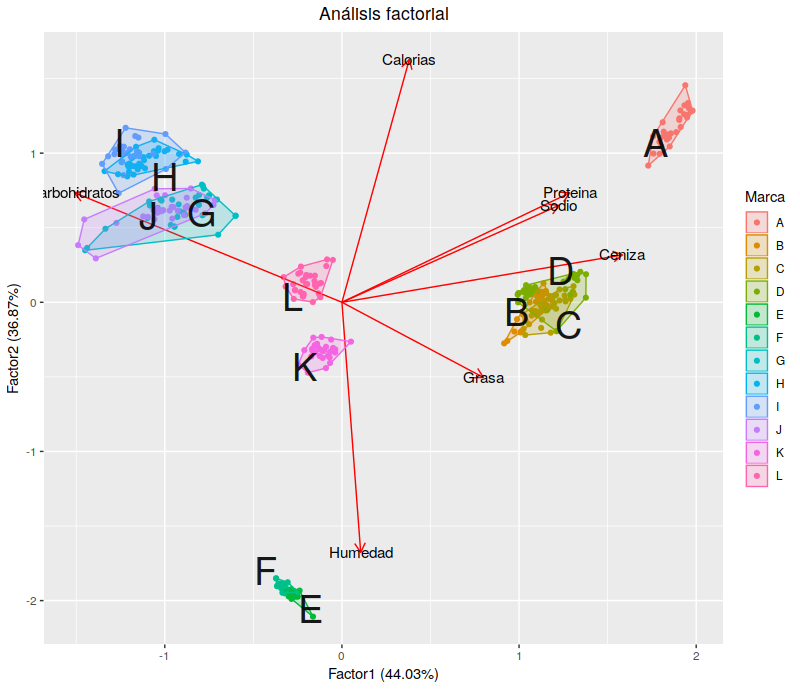
\includegraphics[scale=.35]{images/biplotFactores.png} 
	\label{i_biplot_Factores}
	\caption{Biplot usando 2 factores}
\end{figure}
\end{frame}

\section{Análisis por agrupación.}

\subsection{Elección del número de clusters}

\begin{frame}
\begin{figure}[h]
\centering
	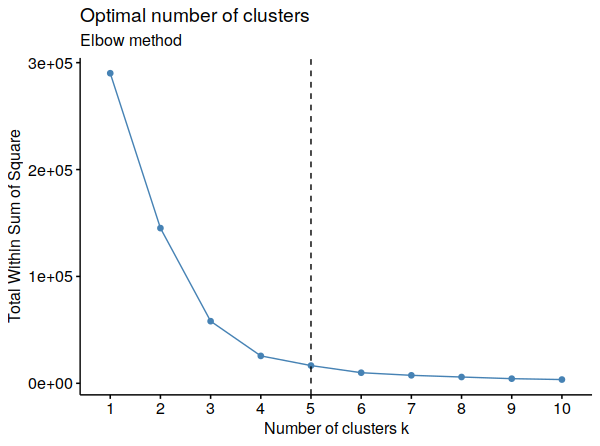
\includegraphics[scale=.5]{images/clusterElbow.png} 
	\label{i_cluster_Elbow}
	\caption{Suma total de cuadrados entre clústers vs número de clusters}
\end{figure}
\end{frame}

\begin{frame}
\begin{figure}[h]
\centering
	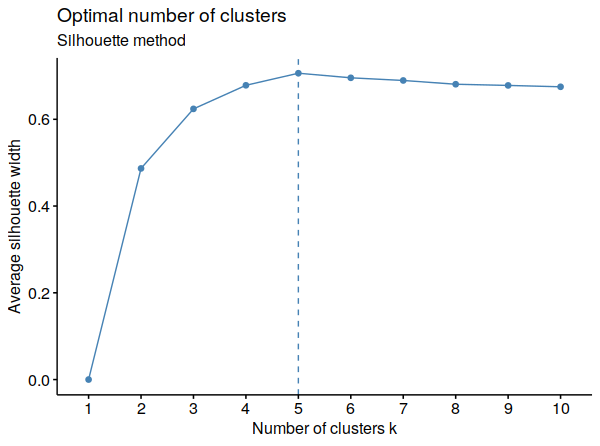
\includegraphics[scale=.5]{images/clusterSilhouette.png} 
	\label{i_cluster_Silhouette}
	\caption{Silhouette promedio vs número de clusters}
\end{figure}
\end{frame}


\subsection{Asignación de clusters}

\begin{frame}
\begin{figure}[h]
\centering
	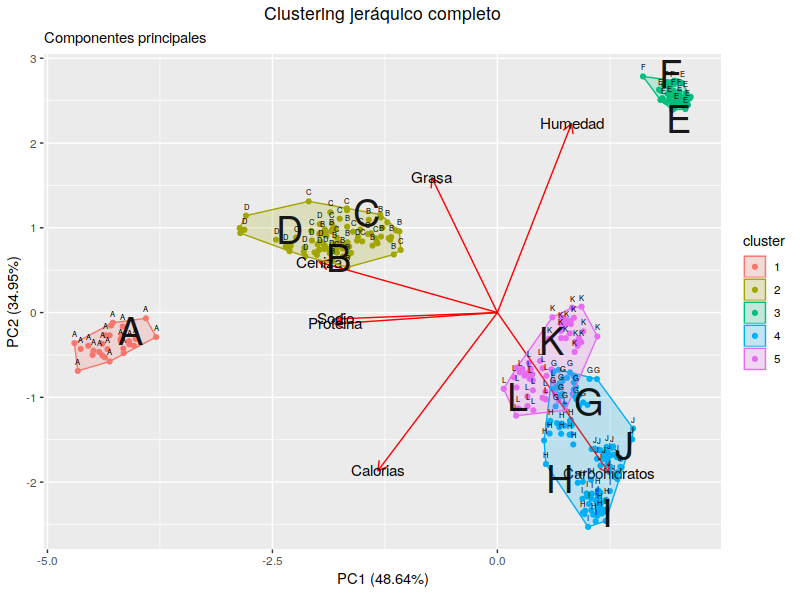
\includegraphics[scale=.35]{images/clusterPCA.png} 
	\label{i_cluster_PCA}
	\caption{Clustering jerárquico completo (Representación: PCA)}
\end{figure}
\end{frame}

\begin{frame}
\begin{figure}[h]
\centering
	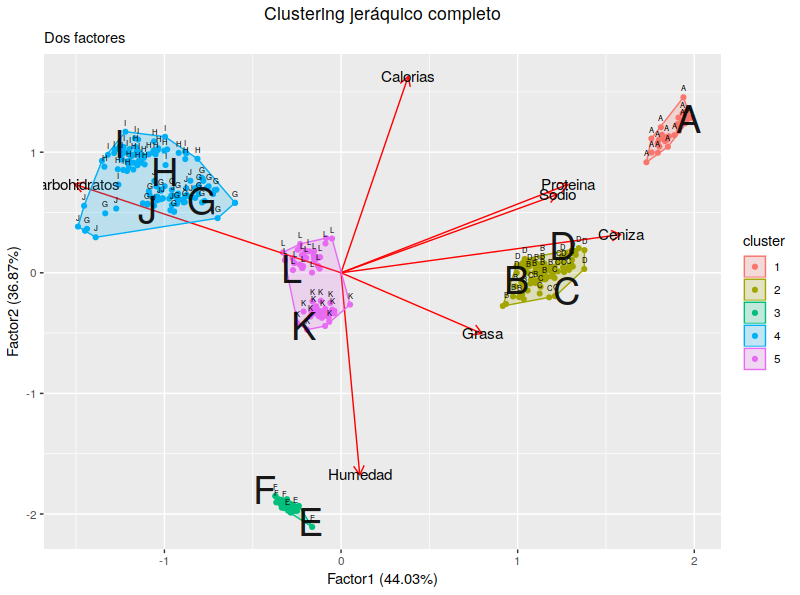
\includegraphics[scale=.35]{images/clusterFactores.png} 
	\label{i_cluster_Factores}
	\caption{Clustering jerárquico completo (Representación: Factores)}
\end{figure}
\end{frame}


\begin{frame}
\end{frame}


\end{document}
